\documentclass[12pt,letterpaper]{article}

\usepackage[spanish,es-noshorthands]{babel}
\usepackage[utf8]{inputenc}
\usepackage[T1]{fontenc}
\usepackage[margin=2.5cm]{geometry}
\usepackage{amsmath}
\usepackage{booktabs}
\usepackage{longtable}
\usepackage{array}
\usepackage{float}
\usepackage{graphicx}
\usepackage{xcolor}
\usepackage{listings}
\usepackage{hyperref}
\usepackage{setspace}
\onehalfspacing
\hypersetup{colorlinks=true,linkcolor=black,urlcolor=blue}

\newcommand{\evidencia}[1]{%
  \fbox{\parbox[c][6.5cm][c]{0.82\textwidth}{\centering\textit{[ESPACIO PARA EVIDENCIA]}\\[0.7em]#1}}%
}

\lstset{
  basicstyle=\ttfamily\small,
  breaklines=true,
  frame=single,
  columns=fullflexible,
  language=R,
  showstringspaces=false
}

\begin{document}

\pagenumbering{gobble}
\begin{titlepage}
\centering
\vspace*{2cm}
{\Large Universidad Nacional de San Agustín de Arequipa\par}
\vspace{0.4cm}
{\large Facultad de Ingeniería de Producción y Servicios\par}
\vspace{0.4cm}
{\large Escuela Profesional de Ingeniería de Sistemas\par}
\vfill
{\Huge\bfseries Análisis descriptivo del ingreso por ventas\par}
\vspace{0.5cm}
{\Large Base de datos \texttt{ventasra1}\par}
\vfill
\begin{flushleft}
\large
\textbf{Asignatura:} Lab. Estadística matemática, probabilidades y métodos empíricos\\[0.4cm]
\textbf{Estudiante(s):} Capatinta Almanza Camilo Bladimir Alexander\\[0.4cm]
\textbf{Docente:} Gonzales Medina Ronny Ivan 
\end{flushleft}
\vfill
{\large Arequipa -- Perú\\2026\par}
\end{titlepage}

\clearpage
\pagenumbering{arabic}
\tableofcontents
\clearpage

\section{Descripción de los datos}

La base de datos original \texttt{ventasra1.sav} fue generada con IBM SPSS Statistics 23. Para el análisis se empleó su versión limpia en formato CSV. La base contiene $10\,711$ casos y 16 variables relacionadas con las ventas de una empresa de ropa. La variable analizada es \texttt{Ingreso\_ventas}, correspondiente al ingreso por ventas.

\section{Metodología}

El procesamiento se realizó en \textit{jamovi}, utilizando el Rj Editor sobre la base en formato CSV. La variable de trabajo se definió como \texttt{x <- data\$Ingreso\_ventas}.

\section{Resultados}

\subsection{Lectura de datos}

\begin{figure}[H]
\centering
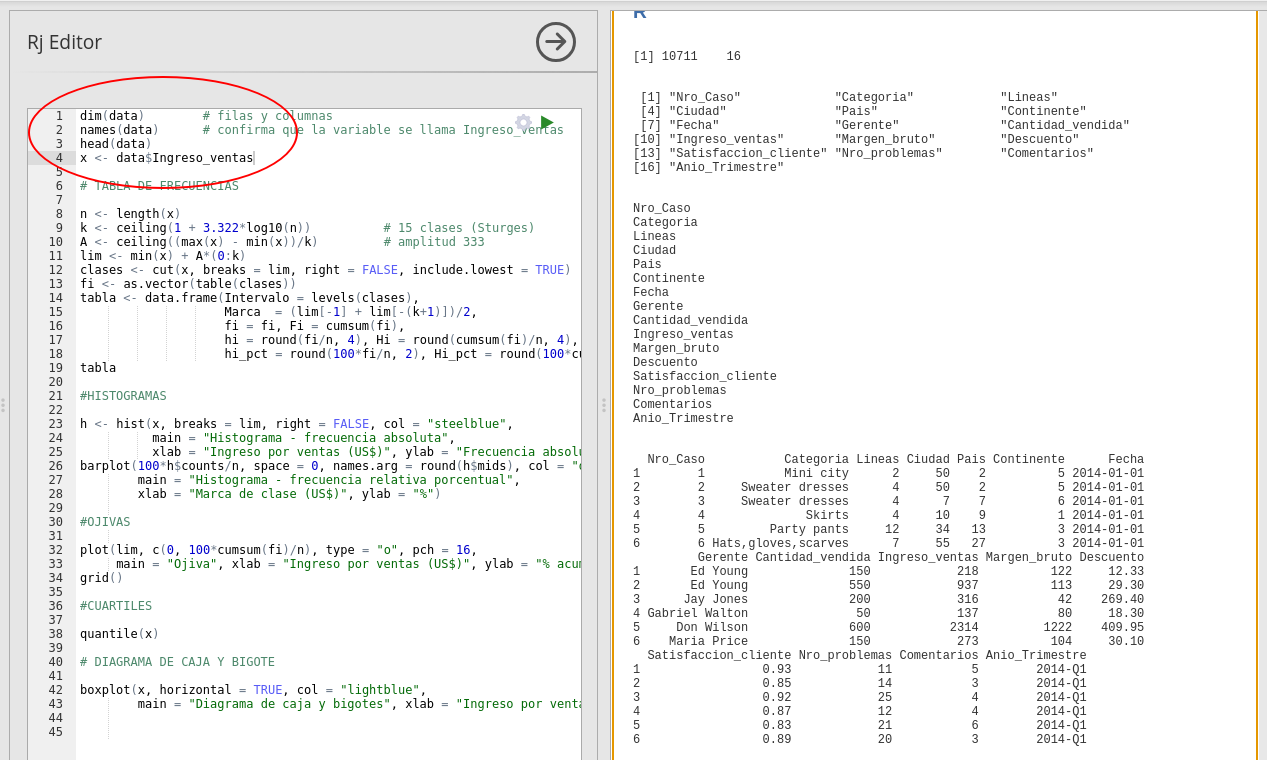
\includegraphics[width=0.82\textwidth]{lectura.png}
\caption{Codigo con ejecución.}
\end{figure}

\subsection{Tabla de frecuencias}

\begin{figure}[H]
\centering
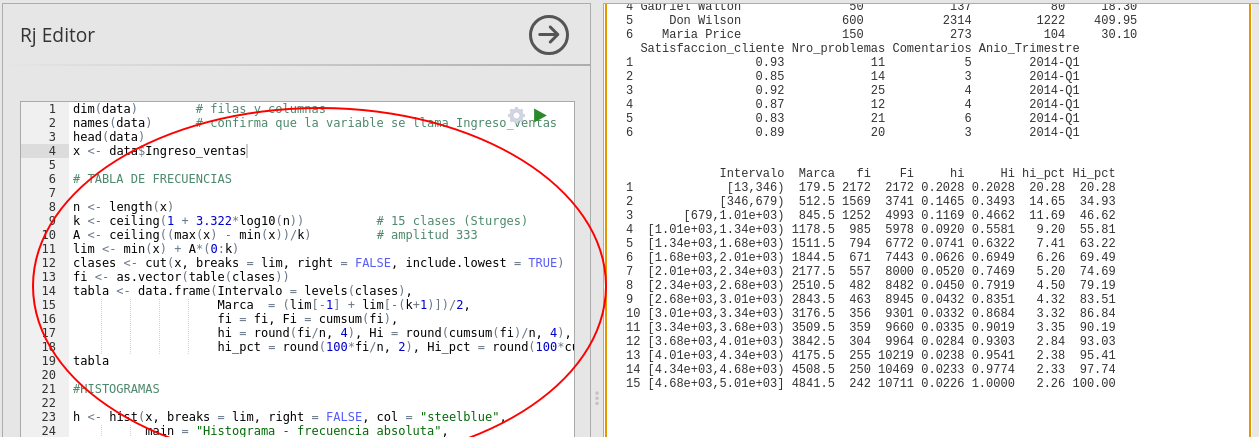
\includegraphics[width=0.82\textwidth]{tabla.png}
\caption{Evidencia de la tabla de frecuencias en jamovi/Rj Editor.}
\end{figure}

\subsection{Histogramas}

\begin{figure}[H]
\centering
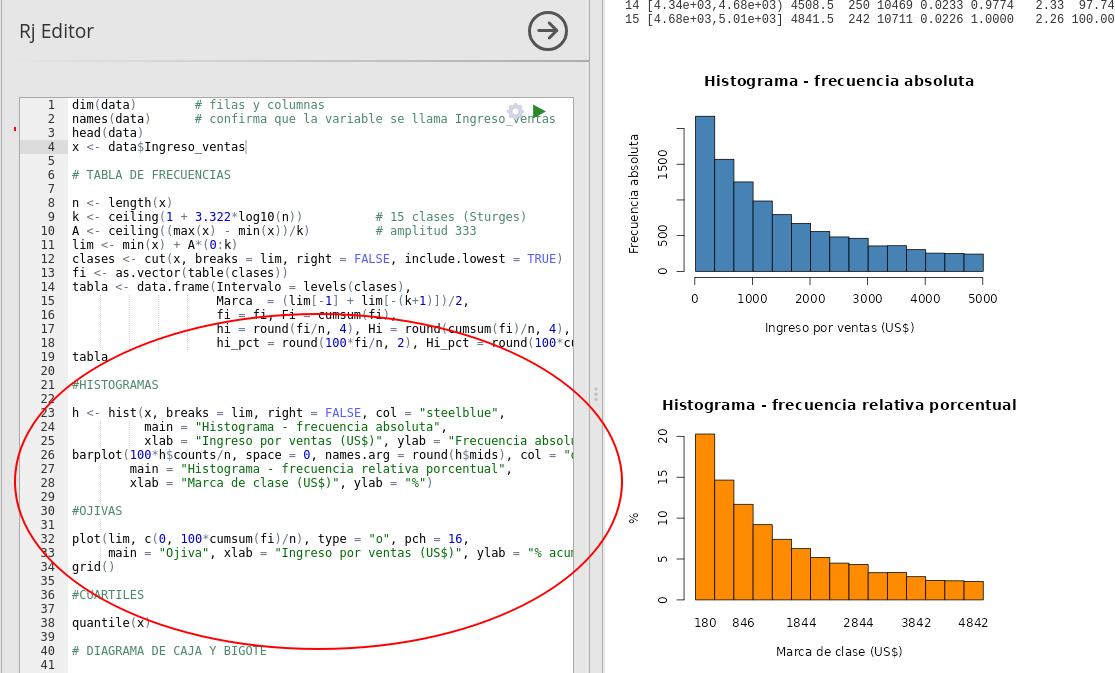
\includegraphics[width=0.82\textwidth]{histo.png}
\caption{Histograma de frecuencia absoluta y frecuencia relativa porcentual.}
\end{figure}

\subsection{Ojiva, cuartiles y diagrama de caja y bigote}

\begin{figure}[H]
\centering
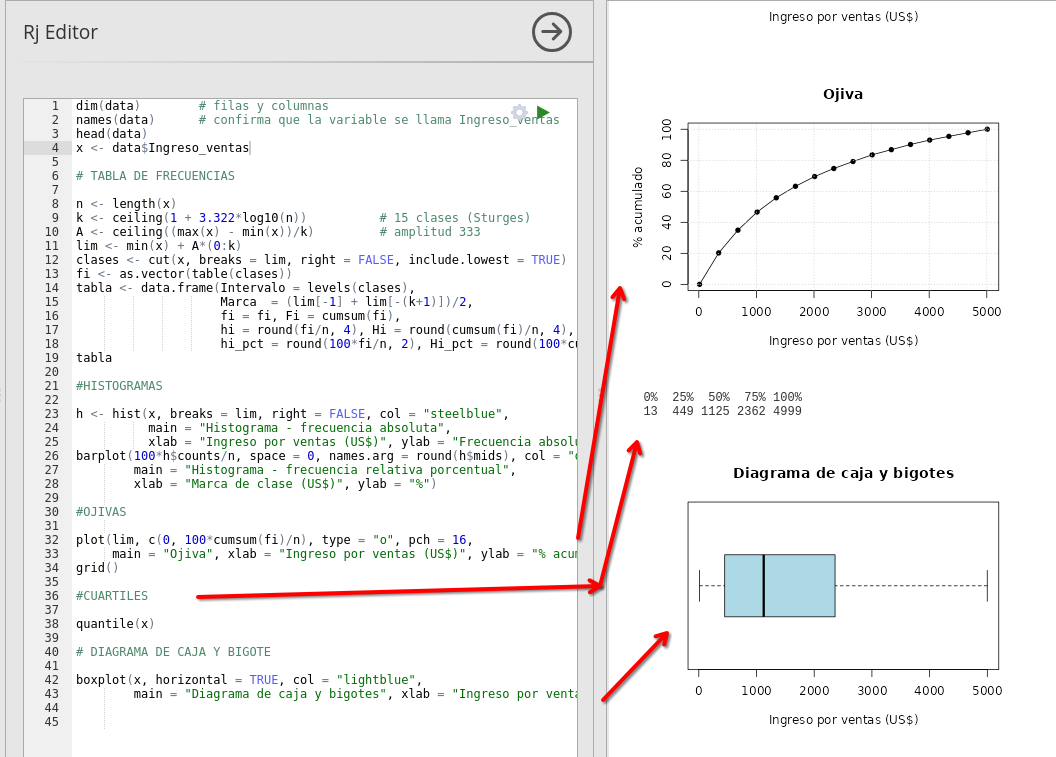
\includegraphics[width=0.82\textwidth]{3.png}
\caption{Ojiva, resumen de cinco puntos y diagrama de caja y bigotes.}
\end{figure}

\section{Interpretación de los resultados}

\subsection{Distribución de frecuencias}

La mayor concentración se encuentra en el intervalo $[13,346)$: 2172 ventas (20.28\%). El 46.62\% de los ingresos es menor que US\$ 1012 y el 90.19\%, menor que US\$ 3676. Desde US\$ 4009, cada intervalo concentra solo entre 2.26\% y 2.38\% de los casos.

\subsection{Histogramas y ojiva}

Las frecuencias disminuyen a medida que aumenta el ingreso y forman una cola hacia los valores altos; por ello, la distribución presenta asimetría positiva. Los dos histogramas conservan la misma forma e intervalos; únicamente cambia la escala: frecuencia absoluta o porcentaje.

La ojiva crece rápidamente en los primeros intervalos y luego se aplana, lo que indica acumulación de ventas pequeñas. El 50\% se alcanza cerca de US\$ 1100, coherente con la mediana de US\$ 1125; el 90\% se alcanza cerca de US\$ 3650.

\subsection{Resumen de cinco puntos y diagrama de caja}

El 25\% de las ventas no supera US\$ 449, el 50\% no supera US\$ 1125 y el 75\% no supera US\$ 2361.5; el máximo es US\$ 4999. El RIC de US\$ 1912.5 y el coeficiente de variación aproximado de 85.5\% muestran alta dispersión. La media (US\$ 1538.92) supera a la mediana, confirmando el sesgo a la derecha.

En el diagrama de caja, la distancia $Q_1$--mediana es US\$ 676 y la distancia mediana--$Q_3$ es US\$ 1236.5; junto con el bigote derecho más largo, esto confirma la asimetría positiva. No hay valores atípicos: todos los datos están dentro de los límites de $1.5\cdot RIC$ (US\$ $-2419.75$ y US\$ 5230.25).

\appendix
\section{Código utilizado en el Rj Editor de jamovi}

El siguiente código permite reproducir la tabla, los gráficos, el resumen de cinco puntos y el diagrama de caja a partir de la base CSV abierta en jamovi.

\begin{lstlisting}
# Paso 1: preparacion
dim(data); names(data); head(data)
x <- data$Ingreso_ventas

# Paso 2: tabla de frecuencias
n <- length(x)
k <- ceiling(1 + 3.322 * log10(n))
A <- ceiling((max(x) - min(x)) / k)
lim <- min(x) + A * (0:k)
clases <- cut(x, breaks = lim, right = FALSE,
              include.lowest = TRUE, dig.lab = 6)
fi <- as.vector(table(clases))
tabla <- data.frame(
  Intervalo = levels(clases),
  Marca = (lim[-1] + lim[-(k + 1)]) / 2,
  fi = fi,
  Fi = cumsum(fi),
  hi = round(fi / n, 4),
  Hi = round(cumsum(fi) / n, 4),
  hi_pct = round(100 * fi / n, 2),
  Hi_pct = round(100 * cumsum(fi) / n, 2)
)
tabla

# Paso 3: histogramas
h <- hist(x, breaks = lim, right = FALSE, col = "steelblue",
          main = "Histograma - frecuencia absoluta",
          xlab = "Ingreso por ventas (US$)",
          ylab = "Frecuencia absoluta")
barplot(100 * h$counts / n, space = 0, names.arg = round(h$mids),
        col = "darkorange",
        main = "Histograma - frecuencia relativa porcentual",
        xlab = "Marca de clase (US$)", ylab = "%")

# Paso 4: ojiva
plot(lim, c(0, 100 * cumsum(fi) / n), type = "o", pch = 16,
     main = "Ojiva", xlab = "Ingreso por ventas (US$)",
     ylab = "% acumulado")
grid()

# Paso 5: resumen de cinco puntos
quantile(x)

# Paso 6: diagrama de caja
boxplot(x, horizontal = TRUE, col = "lightblue",
        main = "Diagrama de caja y bigotes",
        xlab = "Ingreso por ventas (US$)")
\end{lstlisting}

\end{document}
